Time-series prediction of a neural model relies on the input history of equally distributed samples.
\ifthenelse {\boolean{thesis}}{As discussed in earlier chapters, the LSTM model is a recurrent neural network designed to solve the vanishing gradient problem by remembering (preserving) the long dependencies \cite{rasifaghihi_predictive_2020}.}
{The LSTM model is a recurrent neural network designed to solve the vanishing gradient problem by remembering (preserving) the long dependencies~\cite{rasifaghihi_predictive_2020}.}
The cells inside the model act as memory units to preserve the dependence.
Therefore, the output is closely dependent on the previous input samples.
Unlike the normal RNN, and the more modern version GRU, LSTM has a more complicated structure constructed from several logical gates~\cite{LSTM_Hochreiter1997}.
It is the most widely used type of model.
\ifthenelse {\boolean{thesis}}{Chapter~\ref{cha:Analysis} provides a summary of the LSTM cell logic, with corresponding equations explaining the gates logic in detail.} 
{\mbox{Figure~\ref{fig:LSTM-cell2}} provides a summary of the cell logic.
It utilises three gates: forget $f_t$, input $i_t$ and output $o_t$, \mbox{Equation~\ref{eq:LSTM-gates2}}.
The decisions are based around sigmoid $\sigma$ function~\ref{eq:sigmoid2}.
With default $tanh$ as activation function, \mbox{Equation~\ref{eq:LSTM-output2}} describes the procedure for cell state update and further propagation.
Output variables $h_t$ and $c_t$ represent memory cell output and the cell state at timestamp $t$.
\begin{equation}
    \sigma(x) = \frac{1}{1+e^{-x}}
    \label{eq:sigmoid2}
\end{equation}
\begin{figure}[htbp]
    \centering
    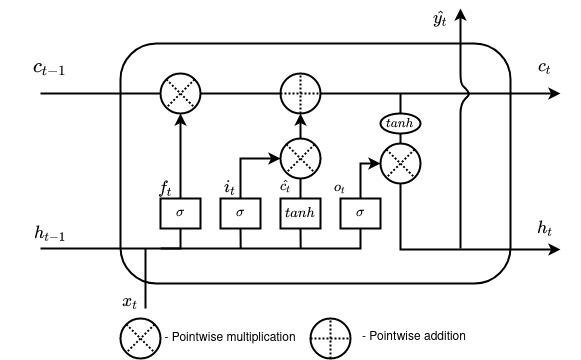
\includegraphics[width=\linewidth]{II_Body/LSTM/images/LSTM.jpg}
    \caption{Long Short-Term Memory Cell}
    \label{fig:LSTM-cell2}
\end{figure}
\begin{equation}
    \begin{split}
        f_t &= \sigma \left(W_f \left[h_{t-1}, x_t \right] + b_f \right) \\
        i_t &= \sigma \left(W_i \left[h_{t-1}, x_t \right] + b_i \right) \\
        o_t &= \sigma \left(W_o \left[h_{t-1}, x_t \right] + b_o \right) \\    
    \end{split}
    \label{eq:LSTM-gates2}
\end{equation}
\begin{equation}
    \begin{split}
        c_t &= f_t c_{t-1}+i_t \times tanh \left(W_c \left[h_{t-1}, x_t \right] + b_c \right) \\
        h_t &= o_t*tanh \left(c_t \right)
    \end{split}
    \label{eq:LSTM-output2}
\end{equation}
}

%
%
The LSTM model has been used widely in stock-price prediction or weather forecasting. 
%? add references if I feel to it
However, unlike State of Charge estimation, which commonly uses $V$, $I$, and $T$ as inputs, those methods utilise the output feature as an input to the subsequent prediction to propagate results further and calculate the time before a critical event occurrence.
Besides, methods like weather forecasting for a week are not limited by lacking output data, since the searched criteria are always known or will be known once they happen, allowing updates and improvements of follow-up predictions.
On the contrast, a battery's actual State of Charge cannot be directly determined or measured making verification against previously-made predictions difficult without additional battery modelling techniques or laboratory equipment.
%, not to mention having it integrated into an Electric Vehicle's accumulator.
It can be determined with a proper battery cycler, performing a set of pulse tests, but this is infeasible for practical applications.
%utilising a battery and affecting its charge and remaining life.
% (As opposed to the SoC estimate, where getting actual values to require a battery cycler capable ... ) 
%%%%%%%%%%%
%Unlike the charge estimation, which can only output a single value based on a history of samples, they are not limited to ... . Therefore, it does not require the output as input since the truth will become known in due time.
As such, to include the charge in the process, SoC as a learning input is used, later making a predicted array of values used on testing.
This introduces potential issues for error accumulation with every evaluation that will be addressed.

%
%
The best way to use the performance of the stateless LSTM model is through training with a data windowing technique.
The NN model will receive a fixed set of equally-distributed time samples at each time prediction.
Every next forecast will shift the time window by a constant step $s$, until all possible combinations of time slices go through the model.
That approach is referred to as a stateless model, which only sees dependencies over input samples rather than preserving every received input, like in stateful implementations.
It also allows the order of the windows to be shuffled to avoid overfitting.
Since no dropout was applied before the model's output, a set of strategies has been applied to update the learning rate and rollback before early stopping to assist the fitting process.
\ifthenelse {\boolean{thesis}}{Chapter~\ref{cha:Analysis} at subsections~\ref{subsec:l-rate} and~\ref{subsec:t_model} explain those two methods, which have already proven to be effective at training SoC models.} 
{Early research on published methods has already utilised those two methods to assist in the models' training process [Sadykov, 1].
It involved a scheduled learning rate value update with every passing epoch for as long as the accuracy kept improving with every passing iteration, as well as assisting the models' recovery in the event of overfitting by double reduction of the value either until the models' return to the same minimal optimisation or finalising the optimum result reach.}
As a result, a NN model will learn dependency between a fixed amount of equally distributed time samples $n$ and yet be independent from the order of the inputs.
\ifthenelse {\boolean{thesis}}{\mbox{Figure~\ref{fig:Windowing}} adapts the earlier Figure~\ref{fig:Windowing3f}, demonstrating how the input dataset is constructed and ordered into a 3-dimensional dataset, with four features (Voltage, Current, Temperature and added initial SoC), 500 timestamps and around a hundred thousand samples to fit on.}
{\mbox{Figure~\ref{fig:Windowing}} demonstrates how the input dataset is constructed and ordered into a 3-dimensional dataset, with four features, 500 timestamps and around a hundred thousand samples to fit on.}
Due to the size of the windows, equivalent to 8 and a quarter minutes of a discharge process, no batching mechanism has been used to reduce computational load and avoid 4-dimensional matrix management.

%
%
\ifthenelse {\boolean{thesis}}{Similar to Chapter~\ref{cha:Analysis}, the mean and standard deviation has been used to normalise all data to speed up the training process.}
{The mean and standard deviation has been used to normalise all data to speed up the training process.}
The normalisation constant from training input samples has been used for all further validation and testing sets to ensure the right trends.
The state of charge narrowed between 0 and 1 to represent the percentage charge to two decimals.
\mbox{Table~\ref{tab:params}} highlights the parameters required to define the initial model, where $s$ defines output step size, which will be justified later in Section~\ref{sec:feed}.
A $\sigma$ function as an output justifies the charge normalisation between 0 and 1.
\ifthenelse {\boolean{thesis}}{The number of neurons has been selected based on the results made in Chapter~\ref{cha:Analysis}, Section~\ref{sec:AN:Results}.
Even though the number of neurons was kept as per the performance result table, only one layer has been utilised due to manual implementation of the model and the inability to validate the multilayer implementation correctness against some published or already-used models.
It was decided to stick to known approaches to validate the efficiency of the newly-proposed technique.
\begin{table}[ht]
    \renewcommand{\arraystretch}{1.3}
    \caption{Model structure and parameters}
    \centering
    \label{tab:params}
    \begin{tabular}{ l l l }
        \hline\hline \\[-4mm]
        Input     & $shape= \left( 1,500,4 \right)$ & $batch=1 $  \\
        \hline
        LSTM      & $activation= 'tanh'$ & $units=131$  \\
        \hline
        Dropout   & $0.0$ &   \\
        \hline
        Output    & $activation= \sigma\left(s, 1 \right)$ &   \\
        \hline\hline
    \end{tabular}
\end{table}
}
{The number of neurons has been selected based on the results made based on earlier discoveries of the most optimal hyperparameters set [Sadykov, 1].
Results were adapted to the new custom-implemented model to validate the technique's efficiency in a comparable way with already-tested approaches.
\begin{table}[ht]
    \renewcommand{\arraystretch}{1.3}
    \caption{Model structure and parameters}
    \centering
    \label{tab:params}
    \resizebox{\columnwidth}{!}{
    \begin{tabular}{ l l l }
        \hline\hline \\[-4mm]
        Input     & $shape= \left( 1,500,4 \right)$ & $batch=1 $  \\
        \hline
        LSTM      & $activation= 'tanh'$ & $units=131$  \\
        \hline
        Dropout   & $0.0$ &   \\
        \hline
        Output    & $activation= \sigma\left(s, 1 \right)$ &   \\
        \hline\hline
    \end{tabular}
    }
\end{table}
}

%
%
\ifthenelse {\boolean{thesis}}
{
The optimisation algorithm for the fitting process has been selected as the regular Adam method, which was highlighted in Chapter~\ref{cha:Analysis}, \mbox{Algorithm~\ref{alg:Adam}}, with the corresponding hyperparameters, \mbox{Table~\ref{tab:uni-hyperparams}}.
The selection of this optimiser is made to allow comparison to two early-created LSTM-based models which use the same optimiser in Chapter~\ref{cha:Analysis}.
}
{
The optimisation algorithm for the fitting process has been defined by Adam, \mbox{Algorithm~\ref{alg:copyAdam}}, with the corresponding hyperparameters on \mbox{Table~\ref{tab:newM-params}}.
%\textcolor{red}{Try to use Robust Adam instead, because why the hell not since I lost one month of my life to implement that cursed algorithm from Javids miss-typed notes? Complete this section with details as per Gareth Javid's implementation if RoAdam will be able to produce a faster fitting.}
\begin{algorithm}\captionsetup{labelfont={sc,bf}, labelsep=newline}
    \caption{Adaptive Moment Estimation (Adam) optimisation}
    \begin{algorithmic}[1]
        \STATE \textbf{Number of input samples} \\ $N\gets length(\textit{input data})$\\
        \STATE \textbf{Size of windows} \\ $S\gets length(V_{i..n})$\\
        \STATE \textbf{Output steps} \\ $O\gets length(V_{i..n})$\\
        \STATE Input: $x_n = [V_{i..n}, I_{i..n}, T_{i..n}, SoC_{(i-1)..(n-1))}]$ \\
        - Shape: $X = (N, S, 4)$
        \STATE Output:$y_n = [SoC_{(n-o)..n}] - $Shape:$Y = (N, O, 1)$
        \STATE Define Loss function: $L$ \\
                Get hyperparameters: $\alpha, \beta_1, \beta_2, \epsilon$
        \WHILE{$W_t \text{ does not converge}$}
        \STATE $t \gets t+1$
        \STATE $g_t \gets \nabla_W L_t (W_{t-1})$ \COMMENT{Obtain gradient}
        \STATE $m_t \gets \beta_1 m_{t-1}+(1-\beta_1) g_t $ \COMMENT{$1_{st}$ moment calculation}
        \STATE $\upsilon_t \gets \beta_2 \upsilon_{t-1}+ \left(1-\beta_2 \right)g^2_t $ \COMMENT{$2_{nd}$ moment calculation \label{alg:Adam-Line-2Moment}}
        \STATE $\hat{m_t} \gets \frac{m_t}{1-\beta^t_1}$ \COMMENT{Corrected $\hat{m_t}$}
        \STATE $\hat{\upsilon_t} \gets \frac{\upsilon_t}{1-\beta^t_2} $ \COMMENT{Corrected $\hat{\upsilon_t}$}
        \STATE $W_t \gets W_{t-1}- \alpha \frac{\hat{m_t}}{\sqrt{\hat{\upsilon_t}}+\epsilon} $ \COMMENT{Update parameters}
        \ENDWHILE
    \end{algorithmic}
    \label{alg:copyAdam}
\end{algorithm}
\begin{table}[htbp]
    \renewcommand{\arraystretch}{1.3}
    \caption{Optimiser Hyper-Parameters}
    \centering
    \label{tab:newM-params}
    \resizebox{\columnwidth}{!}{
    \begin{tabular}{ l l l l l l }
        \hline\hline \\[-3mm]
        $\alpha$ & $\beta_1 $ & $\beta_2$ & $\beta_3$ &  $\epsilon$ \\
        \hline
        Linear         &  &  &  & \\% 0.0000001
        Scheduler      & $0.9$ & $0.999$ & $0.999$ &$10^{-8}$ \\% 0.0000001
        (0.001-0.0001) &  &  &  & \\% 0.0000001
        \hline\hline
    \end{tabular}
    }
\end{table}
}